\documentclass[fleqn]{article}

\usepackage{cmap}
\usepackage[T2A]{fontenc}
\usepackage[utf8]{inputenc}
\usepackage[english,russian]{babel}

\usepackage[12pt]{extsizes}
\usepackage[left=20mm, top=15mm, right=15mm, bottom=15mm, nohead, footskip=10mm]{geometry}

\usepackage{listings}
\usepackage{verbatim}
\usepackage{titlesec}
\usepackage{graphicx}
\usepackage{color}
\usepackage[colorlinks=true,linkcolor=black,anchorcolor=black,citecolor=black,filecolor=black,menucolor=black,runcolor=black,urlcolor=black]{hyperref}

\usepackage{courier}

\usepackage{amsmath,amsfonts,amssymb,amsthm,mathtools}

\usepackage{indentfirst}

\begin{document}
\begin{titlepage}
\newpage
\begin{center}
Министерство цифрового развития, связи и массовых коммуникаций Российской Федерации\\
ФГБОУ высшего образования \\
"Сибирский Государственный Университет Телекоммуникаций и Информатики" (СибГУТИ)

Кафедра прикладной математики и кибернетики
\end{center}
\vspace{9em}
\begin{center}
Курсовая работа \\
по дисциплине <<Структуры и алгоритмы обработки данных>>
\end{center}


\vspace{15em}

\begin{center}
\hfillВыполнил: студент 2 курса группы ИП-012 \\
\hfillМаланов Роман Игоревич \\
\hfillПроверил: доцент кафедры ПМиК \\ 
\hfillЯнченко Елена Викторовна
\end{center}

\vfill

\begin{center}
Вариант 47.
\end{center}

\vspace{3em}

\begin{center}
Новосибирск, 2021
\end{center}
\end{titlepage}

\definecolor{gray}{rgb}{0.3, 0.4, 0.4}

\lstset{
  language=C,
  numbers=left,                   % where to put the line-numbers
  stepnumber=1,                   % the step between two line-numbers.
  numbersep=15pt,                  % how far the line-numbers are from the code
  backgroundcolor=\color{white},  % choose the background color. You must add \usepackage{color}
  showspaces=false,               % show spaces adding particular underscores
  tabsize=2,                      % sets default tabsize to 2 spaces
  breaklines=true,                % sets automatic line breaking
  breakatwhitespace=true,         % sets if automatic breaks should only happen at whitespace
  extendedchars=\true,
  inputencoding=utf8,
  basicstyle=\sffamily\footnotesize,
  commentstyle=\fontseries{lc}\selectfont\itshape\color{gray},
  keywordstyle=\color{blue},
  stringstyle=\ttfamily\color{red},
}

\tableofcontents

\newpage

\section{Постановка задачи}

Хранящуюся в файле базу данных {(база №4 "Населённый пункт")} загрузить в память компьютера в виде списка,
подготовить процедуры вывода на экран по 20 строк (записей) с возможностью отказа от просмотра.

Упорядочить данные, используя метод прямого слияния (Merge sort).
Упорядоченные данные вывести на экран.
Сортировка производится по дате поселения и названию улицы.

Предусмотреть возможность быстрого поиска по ключу в упорядоченной базе,
в результате которого из результатов поиска формируется очередь,
содержимое очереди выводится на экран.

Из записей очереди построить дерево поиска (двоичное Б-дерево) по ключу,
отличному от ключа сортировки (используется поле "Номер дома").
Вывести на экран содержимое дерева и предусмотреть возможность
поиска в дереве по запросу.

Закодировать файл базы данных статическим кодом (кодом Фано),
предварительно оценив вероятности всех встречающихся символов.
Построенный код вывести на экран, вычислить среднюю длину кодового слова
и сравнить её с энтропией исходного файла.

\section{Основные идеи и характеристики применяемых методов}

\subsection{Метод сортировки MergeSort}

Сортировка слиянием (merge sort) -- алгоритм сортировки, который упорядочивает списки
или иные структуры с последовательным доступом к данным.
В основе метода лежит операция слияния серий.

Сложность алгоритма определяется сложностью операции слияния серий.
Асимптотическая оценка сложности: $O(n\log n)$ при $n \to \infty$.

Алгоритм обеспечивает устойчивую сортировку. 
При реализации со списками дополнительной памяти не требует.

\subsection{Двоичный поиск}

Двоичный (бинарный) поиск -- классический алгоритм поиска элемента в отсортированном
массиве, использующий дробление массива на половины.

Оценка сложности алгоритма: $O(\log n)$ при $n\to\infty$.

\subsection{Списки и очереди}

Список -- абстрактный тип данных, реализующий упорядоченный
набор значений.
Списки отличаются от массивов последовательным, а не произвольным
доступом к элементам.

В данной работе используются связные списки и очереди.

Связный список -- это структура данных, представляющая собой конечное множество
упорядоченных элементов, связанных друг с другом посредством указателей.
Каждый элемент содержит поле с данными (или указателем на данные)
и ссылку (указатель) на следующий элемент.

Очередь -- это список, добавление элементов в который допустимо лишь в один
его конец, а извлечение производится с другого конца
(принцип организации FIFO - <<первым пришёл -- первым вышел>>).

Сложность доступа: $O(n)$ при $n\to\infty$.

Сложность добавления элемента: $O(1)$.

\subsection{Вид дерева и поиск}

Двоичное Б-дерево -- вид сильноветвящегося дерева, Б-дерево первого порядка.
Состоит из вершин (страниц) с одним или двумя элементами.
Следовательно, каждая страницм содержит две или три ссылки на поддеревья.

Двоичные Б-деревья представляют собой альтернативу АВЛ-деревьям.
При этом поиск происходит как в обычном дереве.

Сложность поиска в двоичном Б-дереве и в АВЛ-дереве одинакова
по порядку величины ($O(\log n)$).

\subsection{Метод кодирования}

Код Фано -- метод построения почти оптимального кода, для которого $L_{\text{ср.}}~<~H(p1,...,p_n)~+~1$.
Метод заключается в следующем.
Упорядоченный по убыванию вероятностей список букв алфавита источника делится на две
части так, чтобы суммы вероятностей букв, входящих в эти части, как можно
меньше отличались друг от друга. Буквам первой части приписывается 0, а
буквам из второй части – 1. Далее также поступают с каждой из полученных
частей. Процесс продолжается до тех пор, пока весь список не разобьется на
части, содержащие по одной букве.

\section{Описание структур данных и использованных алгоритмов}

\subsection{Использованные структуры данных}

Основные использованные в работе структуры данных,
это структура, описывающая одну строку базы данных
(запись - \verb+struct record+), структуры списка и очереди.

\begin{itemize}
	\item \verb+struct record+

		Описывает элемент базы данных,
		состоящий из полей: ФИО (\verb+person+),
		название улицы (\verb+street+),
		номер дома (\verb"house"),
		номер квартиры (\verb"apt"),
		и дата заселения (\verb"date").

		В коде используется как тип данных 
		\verb+Record+.

	\item \verb+struct node+

		Структура, описывающая элемент списка,
		содержащая указатель на запись в базе данных
		(указатель на тип \verb"Record"), и ссылку на
		следующий элемент списка (реализует односвязный
		список).
		В коде используется как тип данных 
		\verb+List+ и как элемент очереди \verb"Que".

	\item \verb+struct Que+

		Структура, описывающая очередь. Содержит
		элементы-указатели на начало списка
		(\verb"head") и на конец списка (\verb"tail").
		Элементом очереди является структура
		\verb"struct node".

\end{itemize}

%\subsection{Особенности реализации алгоритмов}

\section{Описание программы}

\subsection{Описание подпрограмм}

Программа разбита на модули. Основной файл -- \verb+main.c+, 
в котором программа запускается, содержит функции вывода 
на экран меню, списка записей, очереди, и функции
запуска определённых частей программы.

Функция сортировки, \verb+Que mergeSort(List**, int N, tSortType)+,
расположенная в файле \verb+mergeSort.h+,
принимает на вход список элементов, количество элементов, и тип
сортировки (элемент перечисления \verb"tSortType"). Сортировка изменяет сам список и возвращает созданную очередь для дальнейших
действий в основной программе.

Функция \verb"Que search(Que que, Record** indexArr, int size, int year)"
выполняет бинарный поиск по году \verb+year+ в очереди 
с помощью предварительно созданного индексного массива 
\verb"indexArr".
Создаёт и возвращает очередь из найденных элементов.

Рекурсивная функция \verb"pTree addDBTree(Record*, pTree)",
расположенная в файле \verb"dbtree.h",
принимает на вход указатель на данные, которые необходимо
добавить в дерево, и корень дерева, указатель на элемент
структуры \verb+pTree+ (структура так же описана в файле
\verb"dbtree.h" и кроме указателей на левое и правое
поддерево содержит указатель на список для добавления
одинаковых элементов, чтобы не допускать
потери данных при построении дерева).

Процедура \verb"void fano(float* P, int L, int R, int k, int** C, int* Length)"
выполняет построение кода Фано по массиву вероятностей \verb"float* P".
Изменяет массив с готовыми кодами \verb"int** C" и массив
длин кодов \verb"int* Length".


\newpage

\section{Скриншоты}

\begin{figure}[h!]
	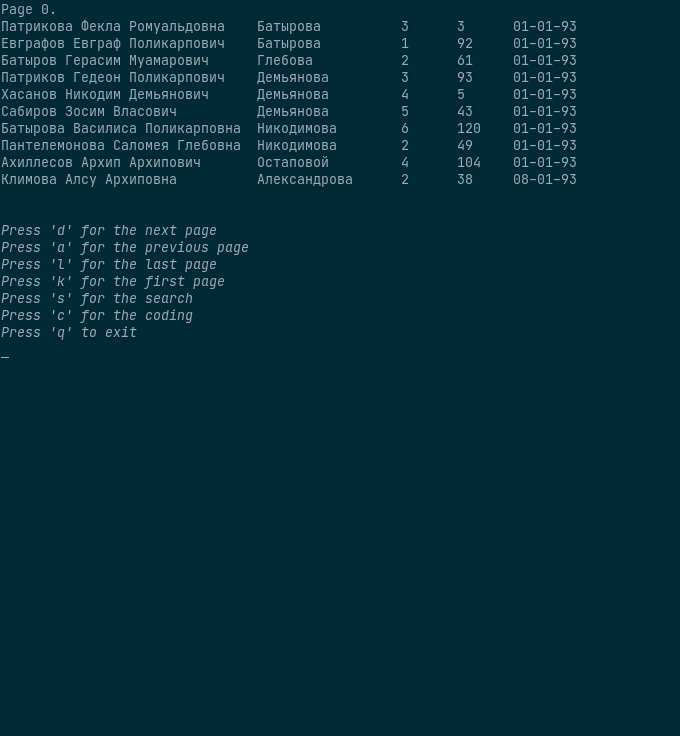
\includegraphics[width=0.5\textwidth]{screen1}
	\caption{Начальное состояние программы. Выведен список записей на экран с возможностью пролистывать записи и запустить подпрограммы}
\end{figure}

\begin{figure}[h!]
	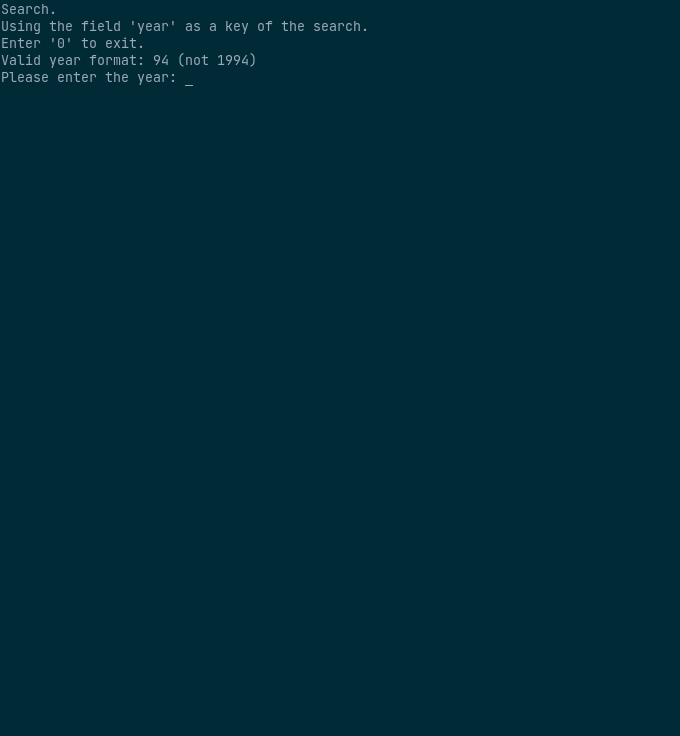
\includegraphics[width=0.5\textwidth]{screen10}
	\caption{Запрос года для запуска поиска}
\end{figure}

\begin{figure}[h!]
	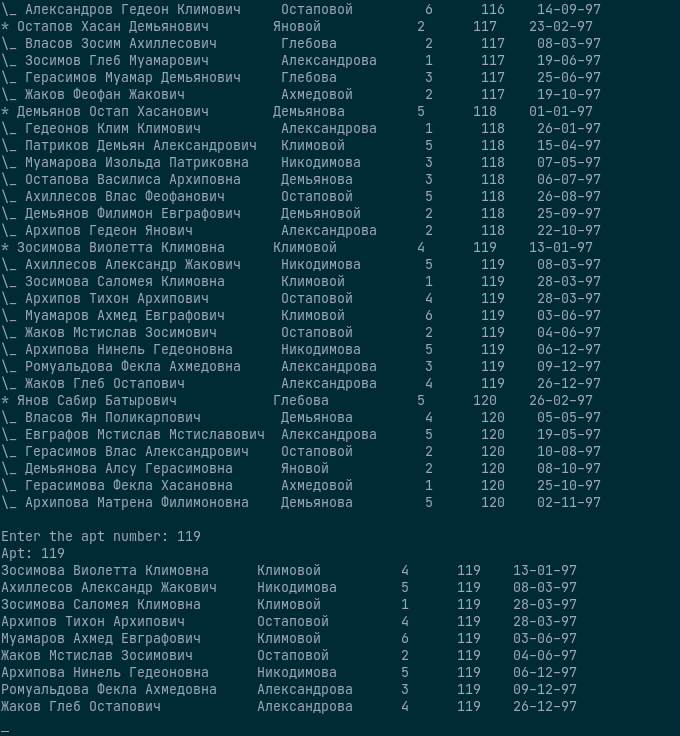
\includegraphics[width=0.5\textwidth]{screen2}
	\caption{Построенное дерево записей и поиск по дереву по номеру квартиры}
\end{figure}

\begin{figure}[h!]
	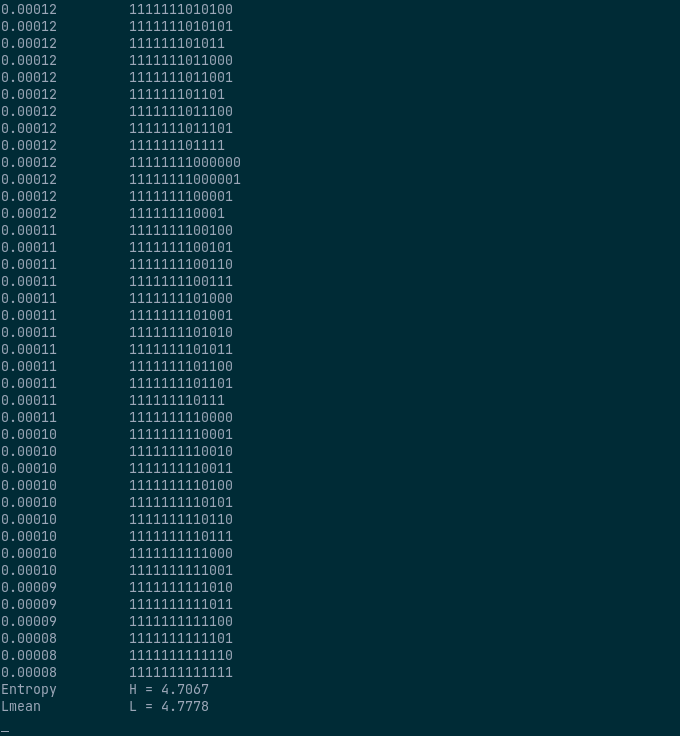
\includegraphics[width=0.5\textwidth]{screen3}
	\caption{Построенный код Фано для файла базы данных}
\end{figure}

\newpage

\section{Выводы}

В результате была реализована программа, считывающая базу
данных из файла, с возможностью сортировки записей, 
поиска по базе, построения дерева, поиска по построенному
дереву, и кодировки файла базы методом Фано.

\newpage

\section{Код программы}

language: C

\lstinputlisting[title=struct.h]{struct.h}
\lstinputlisting[title=list.h]{list.h}
\lstinputlisting[title=que.h]{que.h}
\lstinputlisting[title=search.h]{search.h}
\lstinputlisting[title=mergeSort.h]{mergeSort.h}
\lstinputlisting[title=insertSort.h]{insertSort.h}
\lstinputlisting[title=dbtree.h]{dbtree.h}
\lstinputlisting[title=fano.h]{fano.h}
\lstinputlisting[title=coding.h]{coding.h}

Source-файлы:
\lstinputlisting[title=main.c]{main.c}

\end{document}
